\subsection{Le recyclage, une obligation}

Le recyclage est défini par le Larousse  comme étant l'\og{}\textit{Ensemble des techniques ayant pour objectif de récupérer des déchets et de les réintroduire dans le cycle de production dont ils sont issus}\fg{}. L'un des objectifs de l'Europe est de réduire les déchets. Une série de lois ont donc été adoptées par l'union européenne, puis retranscrite par la France. 

La directive européenne 2012/19/UE du 4 juillet 2012, retranscrite dans le droit français par le décret 2014-928 du 19 août 2014 oblige de plus les magasins dont la surface est supérieure à $400m^2$ à accepter n'importe quel \textit{DEEE} de petite taille, et ce sans obligation d'achat. 

Depuis 2005, un décret (articles R. 543-172 à R. 543-206 du code de l'environnement) mis en place pour répondre aux directive européenne oblige le consommateur à recycler un objet électronique lorsqu'il en achète un nouveau. Pour ce faire, il peut le ramener soit dans le lieu d'achat du nouveau, soit en déchetterie, soit dans les réseaux solidaire comme Emmaüs.

\begin{wrapfigure}{l}{0.3\linewidth}
~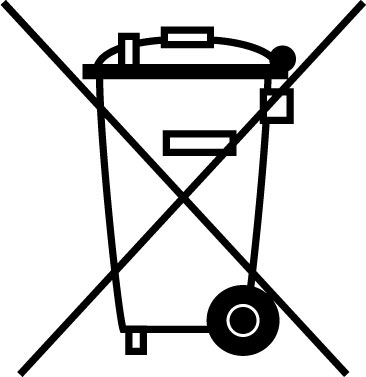
\includegraphics[scale=0.33]{Rsc/pictopoubellebarree.jpg} 
\end{wrapfigure} 
La loi a également mis en place le pictogramme représentant une poubelle barrée, présent sur chaque objet électronique. Il indique que le produit doit être recyclé en fin de vie. 

Plus flagrant peut être, la loi a mis en place la taxe d'éco-participation. Celle ci rend le consommateur contributeur du recyclage. Elle est calculée à partir du coup de collecte du produit (donc de son poids et de sa taille) et du coup de traitement. Ainsi, les prix varient de un centime d'euro pour un \textit{GPS} à 13\euro pour un congélateur. 

L'argent est directement payée par le consommateur. Elle est collectée par le distributeur (\textit{but},\textit{carrefour}, \dots). Une partie de l'argent est donnée aux constructeurs, qui acceptent les \textit{DEEE},le reste est donné aux éco-organisme. 

Les éco-organismes sont divisés en trois entités différentes : les organismes de collecte, les organismes de traitement et les organismes de remise en état. Ces trois types différent vont toucher une division correspondant au service fourni lors du recyclage. 

\medbreak

L'association \textit{Envie 44} basée à Nantes, dont le directeur adjoint, Christophe Roudon, a été interviewé par en 2008 \textit{7\&CO}, une émission de la chaine de télévision \textit{Télénantes}. Il affirme toucher 20\% de ses recettes grâce aux subventions de l'état. 

Cette firme est un réseau solidaire. Elle récupère les \textit{DEEE} auprès des producteurs de déchets électroniques (principalement des administration : mairie, hôpital) et se chargent du recyclage. 

Pour \textit{Envie 44}, le recyclage se divise en deux parties. 
\begin{itemize}
\item 12\% des DEEE étaient rénovés en 2008. Il estimait alors que ce taux pourrait monter jusqu'à 25\%, mais pas plus : 3 machines sont nécessaire pour en réparer une. En 2014, l'entreprise a vendu plus de 7000 articles issus du recyclage. 
\item le reste est envoyé dans des centres de traitement, à Rennes et à Angers.
\end{itemize}

Pour l'entreprise, l'éco-participation a été un véritable moteur, qui lui a permis de se développer. Elle compte aujourd'hui 92 employés. De nombreuses entreprises de recyclage ont étés fondées à la suite du décret. 